\section{Discussion}

In this work, we sought to objectively compare the robustness and user
preference of the neuromuscular and impedance control strategies for powered,
robotic knee and ankle prostheses. Overall, we found that users rated the
neuromuscular control more highly than impedance control and using impedance
control led to significantly more falls compared to walking without a
prosthesis. While the median number of falls accrued by impedance control across
all subjects in both the undisturbed and disturbed conditions was higher than
those of neuromuscular control, these differences were not significant. The only
measure of gait stability in which a significant difference between the
neuromuscular and impedance controllers was measured was the torso pitch
variability, which neuromuscular control significantly reduced in the
disturbance case compared to impedance control.

Categorizing the falls by their type gives more insight into differences between
the controllers. There were reasons for falls with each controller that did not
exist for the other. For NM control, missed transitions between stance and swing
caused three falls. While these falls could be directly attributed to the
leg-angle threshold in the high level state machine that governs the
stance/swing state transition (\cref{fig:stance_swing_state_machine}), that
these falls only occurred with neuromuscular control suggests a causal
difference in the two strategies. One possible important difference between the
implemented neuromuscular and impedance control strategies was that impedance
control typically provided much more ankle push of work, as shown in
\cref{fig:treadmill_exp_ankle_work}. In impedance control, the transition
transition to the third phase of gait generates a large burst of ankle power,
which users may interpret as a signal that the prosthesis is ready to enter
swing. In contrast, neuromuscular control may not have provided any such signal
due to the lack of ankle work. It is possible that such cues to the user should
be explicitly considered in the design of prosthesis controllers, especially
when they can help inform correct transition of discrete state.
\begin{marginfigure}
    \centering 
    %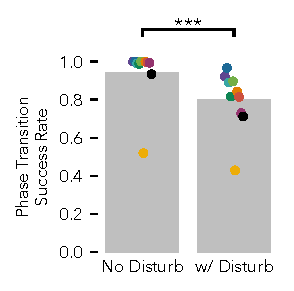
\includegraphics[width=\textwidth]{phase_success}
    \missingfigure[figwidth=\textwidth]{ankle work}
    \caption{Normal Walking, impedance and neuromuscular control ankle
    work.}\label{fig:treadmill_exp_ankle_work}
\end{marginfigure}

Impedance control suffered from two failure modes specific to the structure of
its stance finite state machine. The first failure mode, missed transitions
between the second and third phases of stance, occurred if the user did not
dorsiflex the ankle enough to trigger the transition. This failure often
led to trips during swing or a later loss of balance. In contrast, the knee
collapse failure mode happened if the impedance controller switched to the third
phase of stance too early, which could cause a sudden reduction in knee
extension torque. The fact that individual subjects fell for both of these
reasons suggests that we cannot fix these faliure modes by simply tuning the
ankle angle threshold. Decreasing the threshold to prevent missed transitions
would likely cause more knee collapses. Conversely, increasing the threshold
would likely cause more missed transitions. 

Finally, users suffered from trips during swing when using both stance control
strategies, which were both paired with the same minimum-jerk trajectory
generation swing control strategy. However, these trips occurred three times
more frequently with impedance stance control than with neuromuscular stance
control. Many of the trips that occurred with impedance control were preceded by
a missed transition between the second and third stance phases. Neuromuscular,
control, in contrast, is smooth throughout stance with no discrete transitions,
and thus may allow for a smoother transition to swing and fewer swing trips.
Nonetheless, even with its smoother stance phase, subjects still tripped during
swing several times with the Neuromuscular control. Therefore, in
\cref{sec:swing_control_planning} we seek to explicitly minimize the risk of
falling by using an estimate of the current and future trajectories of the hip
height and orientation to plan knee and ankle swing trajectories that avoid
premature ground contact.

The smooth stance phase of the neuromuscular model, which eliminates failure
modes such as knee collapses and missed stance phase transitions, and may help
reduce swing trips, comes at the cost of dramatically increased model
complexity. The implemented impedance controller has 20 parameters: 3 stance
phases $\times$ 2 joints $\times$ 3 parameters per joint per phase $+$ 2
transition parameters. In contrast, the implemented neuromuscular control is
more than 4 times as complex as it has 80 parameters: 54 defining
muscle-specific mechanical properties, 9 defining shared muscle properties, and
17 defining the neural reflexes. 

Of these 80, we chose to only optimize 18 when generating parameter the sets in
order to avoid local minimum and to complete the optimization in a reasonable
amount of time. The choice of which 18 parameters to choose was based on trial
and error. In the clinical setting, this lack of transparency about the function
of and interdependencies between these 80 parameters may make practical
application of neuromuscular control difficult.  Therefore, in order to achieve
the potential benefits of a smooth controller that does not have discrete stance
phases, while avoiding excessive complexity, in \cref{sec:phase_estimation}, we
explore an alternative approach to stance control. This approach relies on a
continuous estimate of phase and easily interpretable models for the output
behavior as a function of phase.

A surprising result of this experiment is the lack of substantial differences
between suboptimal and optimal controllers. Only the in the case of impedance
control under disturbances did the user unanimously restate their preference for
the control parameter sets they had preferred on the optimization day. The lack
of clear differences between the neuromuscular parameter sets could be the
result of the neuromuscular model generally being less sensitive to its
parameters than the impedance controller. For example, large differences in
behavior between impedance control parameter sets can result if one set of
parameters causes many missed phase transitions and another parameter set does
not. Another reason for the lack of clear difference in user ratings could be
the difference in the query. During the optimization procedure, subjects were
asked to directly prefer one controller to other after short
$\unit[\sim10]{sec}$ bouts of walking on each control. In contrast, on the data
collection day, controllers were independently rated on a 1-10 scale after 2
minutes of walking. In future work, we should check for consistency of the
preferred parameters by performing the dueling bandits optimization procedure on
multiple days in order to see if the users preferences are consistent from day
to day.

Finally, our simulated results presented in \cref{sec:control_sim} predicted a
larger difference between controllers that was not borne out by this experiment.
In future work, the motion capture data collected during these trials should be
used to improve the neuromuscular model so that researchers can perform
experiments investigating prosthetic device performance with a higher likelihood
that those results translate to the real world. Such predictive models would
vastly reduce the time it takes to iterate on prosthesis controllers.
